\chapter{Experiments and Results}
\label{chapter:ref}

\section{Dataset}

This study utilizes a dataset provided by a hospital, containing 5,860 records from periodic patient examinations. The dataset includes data from 412 patients and is categorized into three types of data to support the analysis: constant data, serial data, and output data. Furthermore, the data is divided into two subsets based on the type of vascular access: Arteriovenous Fistula (AVF) and Arteriovenous Graft (AVG).

\subsection{Input Data}

\begin{enumerate}
  \item \textbf{Constant Input (Clinical Features)}: The constant input includes patient-specific clinical characteristics, which remain consistent over time. The selected features for this study are as follows:
  \paragraph{Demographics}:
  \begin{itemize}
    \item \textbf{Age}
    \item \textbf{Gender}
  \end{itemize}
  \paragraph{Comorbidities}:
    \begin{itemize}
    \item \textbf{Diabetes Mellitus (DM)}
    \item \textbf{Hypertension (HTN)}
    \item \textbf{Dyslipidemia (Dyslipid)}
    \item \textbf{Coronary Artery Disease (CAD)}
    \item \textbf{Acute Myocardial Infarction (AMI)}
    \item \textbf{Cerebral Vascular Accident (CVA)}
    \item \textbf{Peripheral Artery Occlusive Disease (PAOD)}
    \item \textbf{Heart Failure (HF)}
  \end{itemize}
  
  These features capture the clinical background of the patient, providing valuable context for predicting procedural outcomes.
  \item \textbf{Serial Input (Procedural Features)}: The serial input focuses on vascular access-related features that vary over time. The selected features include:
  \begin{itemize}
    \item \textbf{Location of the Access Site}
    \item \textbf{Type of Vascular Access (AVF or AVG)}
    \item \textbf{QA value}: A clinical measurement indicative of vascular access functionality.
  \end{itemize}
\end{enumerate}

By combining these features with constant inputs, the dataset offers a comprehensive representation of both static and dynamic aspects of patient health. Additionally, the dataset is divided into two subsets based on the "Type of Vascular Access":

\begin{itemize}
    \item \textbf{Arteriovenous Fistula (AVF) Dataset}
    \item \textbf{Arteriovenous Graft (AVG) Dataset}
\end{itemize}

\subsection{Output Data}
The output data represents the procedural outcome, specifically whether the patient underwent a percutaneous transluminal angioplasty (PTA). The label is determined based on the following two features:

\begin{itemize}
    \item \textbf{PTA\_S (Simple PTA)}: Indicates that the PTA procedure addressed only a single site of stenosis.
    \item \textbf{PTA\_C (Complex PTA)}: Indicates that the PTA procedure addressed two or more sites of stenosis.
\end{itemize}

The final label, PTA, is derived by considering the union of these two features, effectively capturing all cases where a PTA procedure was performed, regardless of its complexity.

\subsection{Data Organization}
To ensure consistency and clarity:

\begin{itemize}
    \item The dataset contains 5,860 records collected from 412 patients during regular clinical monitoring.
    \item Constant input features (clinical data) and serial input features (vascular access data) are combined for each patient.
    \item Based on the "Type of Vascular Access," all data is stratified into two groups:
    \begin{itemize}
        \item \textbf{Arteriovenous Fistula (AVF)}: For patients with native fistulas.
        \item \textbf{Arteriovenous Graft (AVG)}: For patients with synthetic grafts.
    \end{itemize}
\end{itemize}

This structured dataset provides a solid foundation for building machine learning models that incorporate both clinical and procedural data to predict procedural outcomes effectively.

To better understand the distribution of patients in the dataset, we analyzed the proportions of patients with Arteriovenous Fistula (AVF) and Arteriovenous Graft (AVG), as well as the distribution of patients who underwent Percutaneous Transluminal Angioplasty (PTA) procedures.

\begin{figure}[H]
    \centering
    \begin{subfigure}[b]{0.4\textwidth}
        \centering
        \includegraphics[width=\linewidth]{figures/Type of patient’s vascular access.png}
        \caption{Type of patient’s vascular access}
        \label{fig:vascular-access}
    \end{subfigure}%
    \hfill
    \begin{subfigure}[b]{0.6\textwidth}
        \centering
        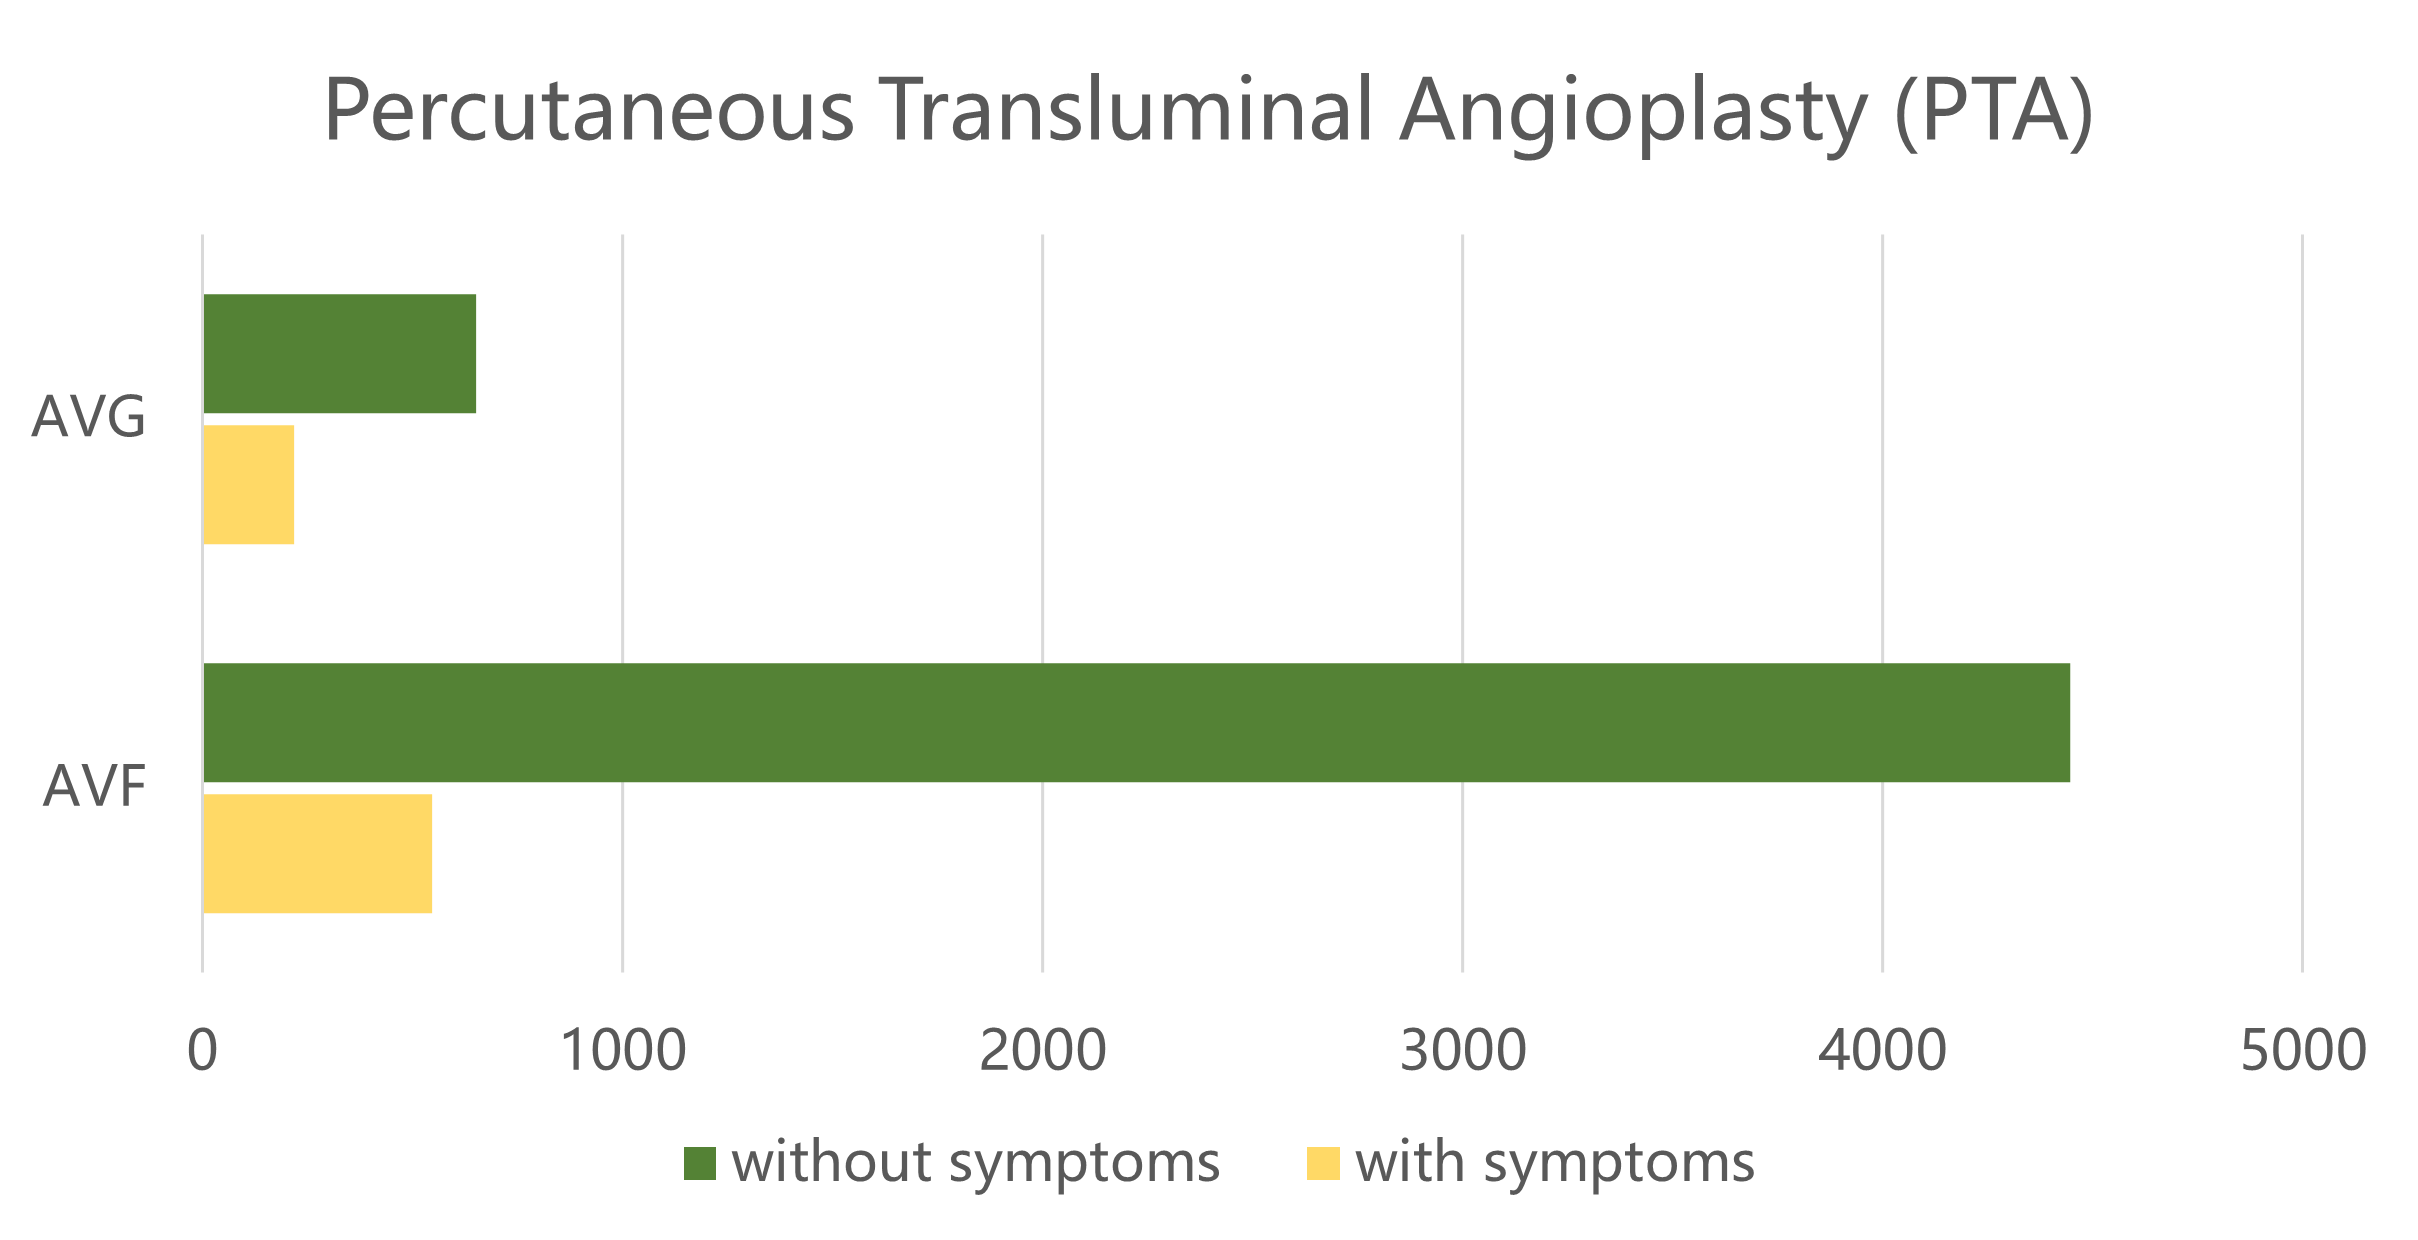
\includegraphics[width=\linewidth]{figures/PTA symptom distribution.png}
        \caption{PTA symptom distribution}
        \label{fig:pta-symptom}
    \end{subfigure}
    \caption{Overview of patient data}
    \label{fig:combined}
\end{figure}

Figure 4.1(a) illustrates the distribution of the dataset based on the type of vascular access. Among the 5,860 records, 85.1\% (4,991 records) belong to patients with AVF, while 14.9\% (869 records) are from patients with AVG. This highlights a significant predominance of AVF cases in the dataset, with AVF records outnumbering AVG records by approximately 6 times. Figure 4.1(b) shows the distribution of patients who underwent PTA procedures, further divided into those with and without symptoms. For AVF patients, the majority did not undergo surgery, with 4,445 (89.1\%) cases categorized as "no PTA," while 546 (10.9\%) cases underwent PTA. Among those who underwent PTA, the majority were asymptomatic. For AVG patients, 651 (74.9\%) cases did not undergo PTA, while 218 (25.1\%) cases underwent PTA. Similar to AVF, most AVG patients who underwent PTA procedures were asymptomatic. However, the proportion of AVG patients undergoing PTA (25.1\%) is significantly higher compared to AVF (10.9\%). The data highlights the disparity in procedural intervention rates between the two vascular access types. AVF patients appear less likely to undergo PTA compared to AVG patients. 

These visualizations emphasize the diversity of patient profiles in the dataset and provide a foundation for the analysis and modeling performed in subsequent sections.
\newpage
\section{Feature Engineering}

To ensure the dataset is suitable for analysis and accurately represents the clinical scenarios, two feature engineering methods were applied: Data Alignment and Feature Creation. These steps enhance the model's ability to capture meaningful patterns and improve prediction performance.

\subsection{Data Alignment}

In the original dataset, there is no Qa value recorded for the day of surgery. Instead, the dataset provides the difference in days between the current record and the previous one. To address this, the record immediately preceding the surgery was selected to represent the surgical day. This approach aligns the data temporally, ensuring that the features used in the model correspond to the patient's most recent clinical status before the procedure. Figure 4.2(b) illustrates the data alignment process.

\begin{figure}[H]
    \centering
    \begin{subfigure}[b]{0.5\textwidth}
        \centering
        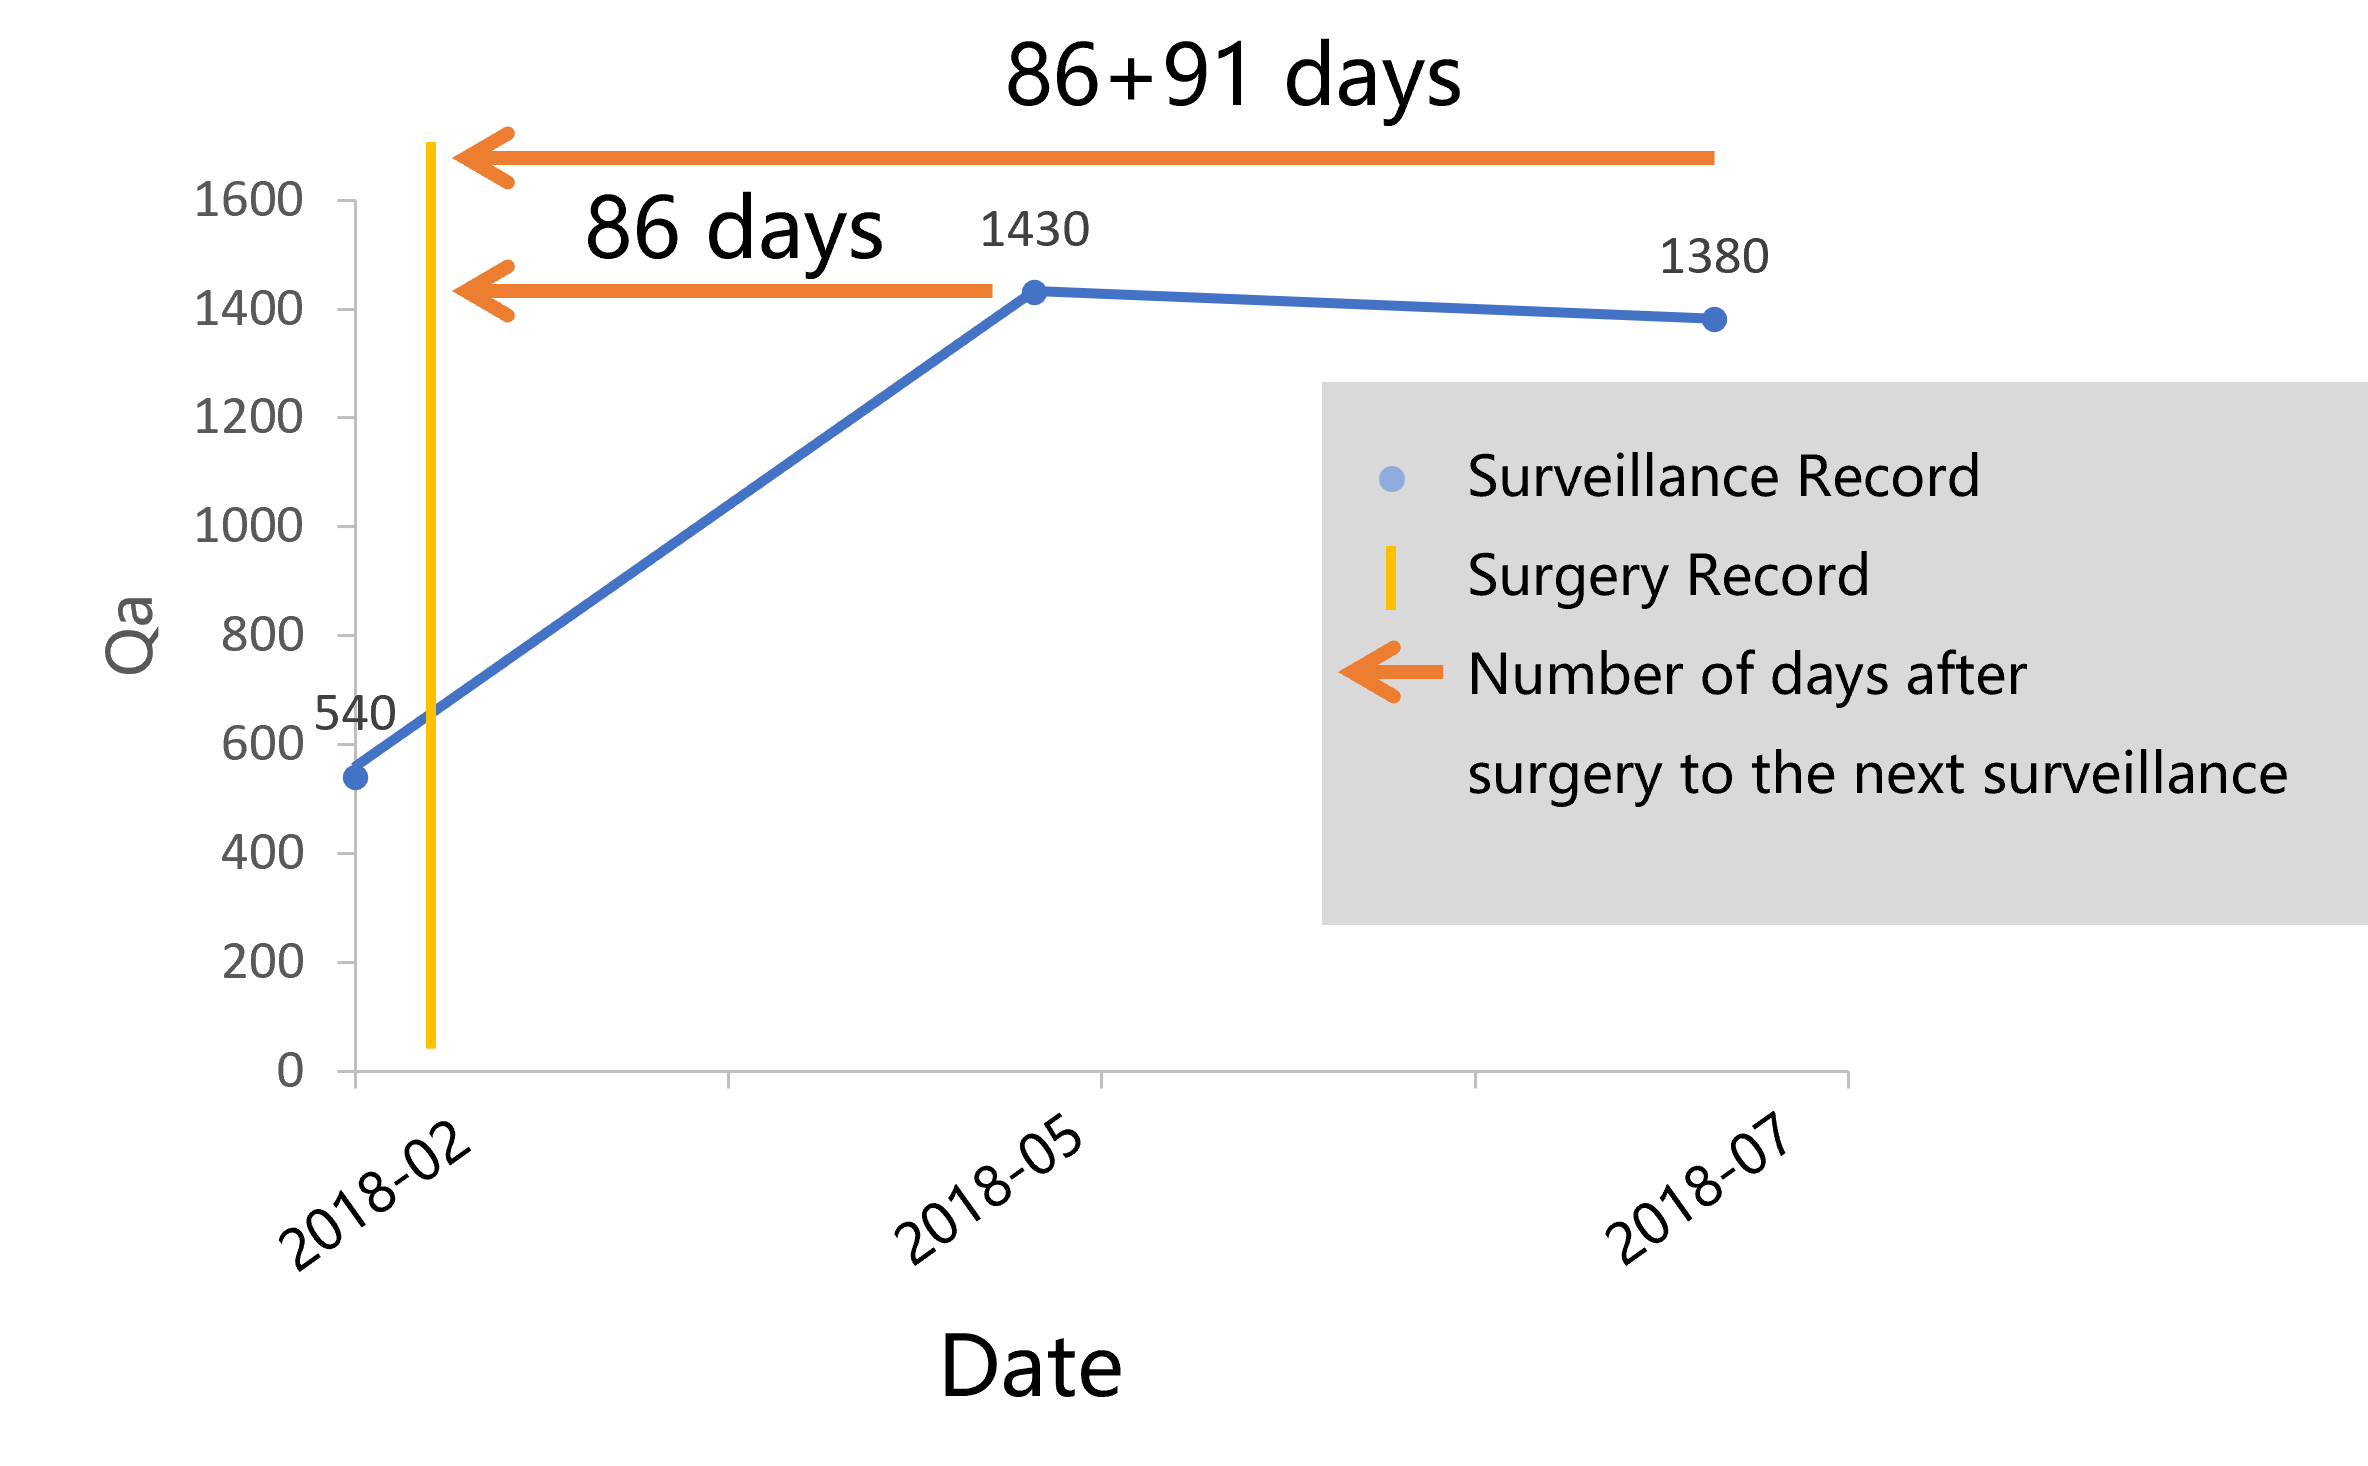
\includegraphics[width=\linewidth]{figures/Patient surveillance and surgery records.png}
        \caption{Patient surveillance and surgery records}
        \label{fig:vascular-access}
    \end{subfigure}%
    \hfill
    \begin{subfigure}[b]{0.4\textwidth}
        \centering
        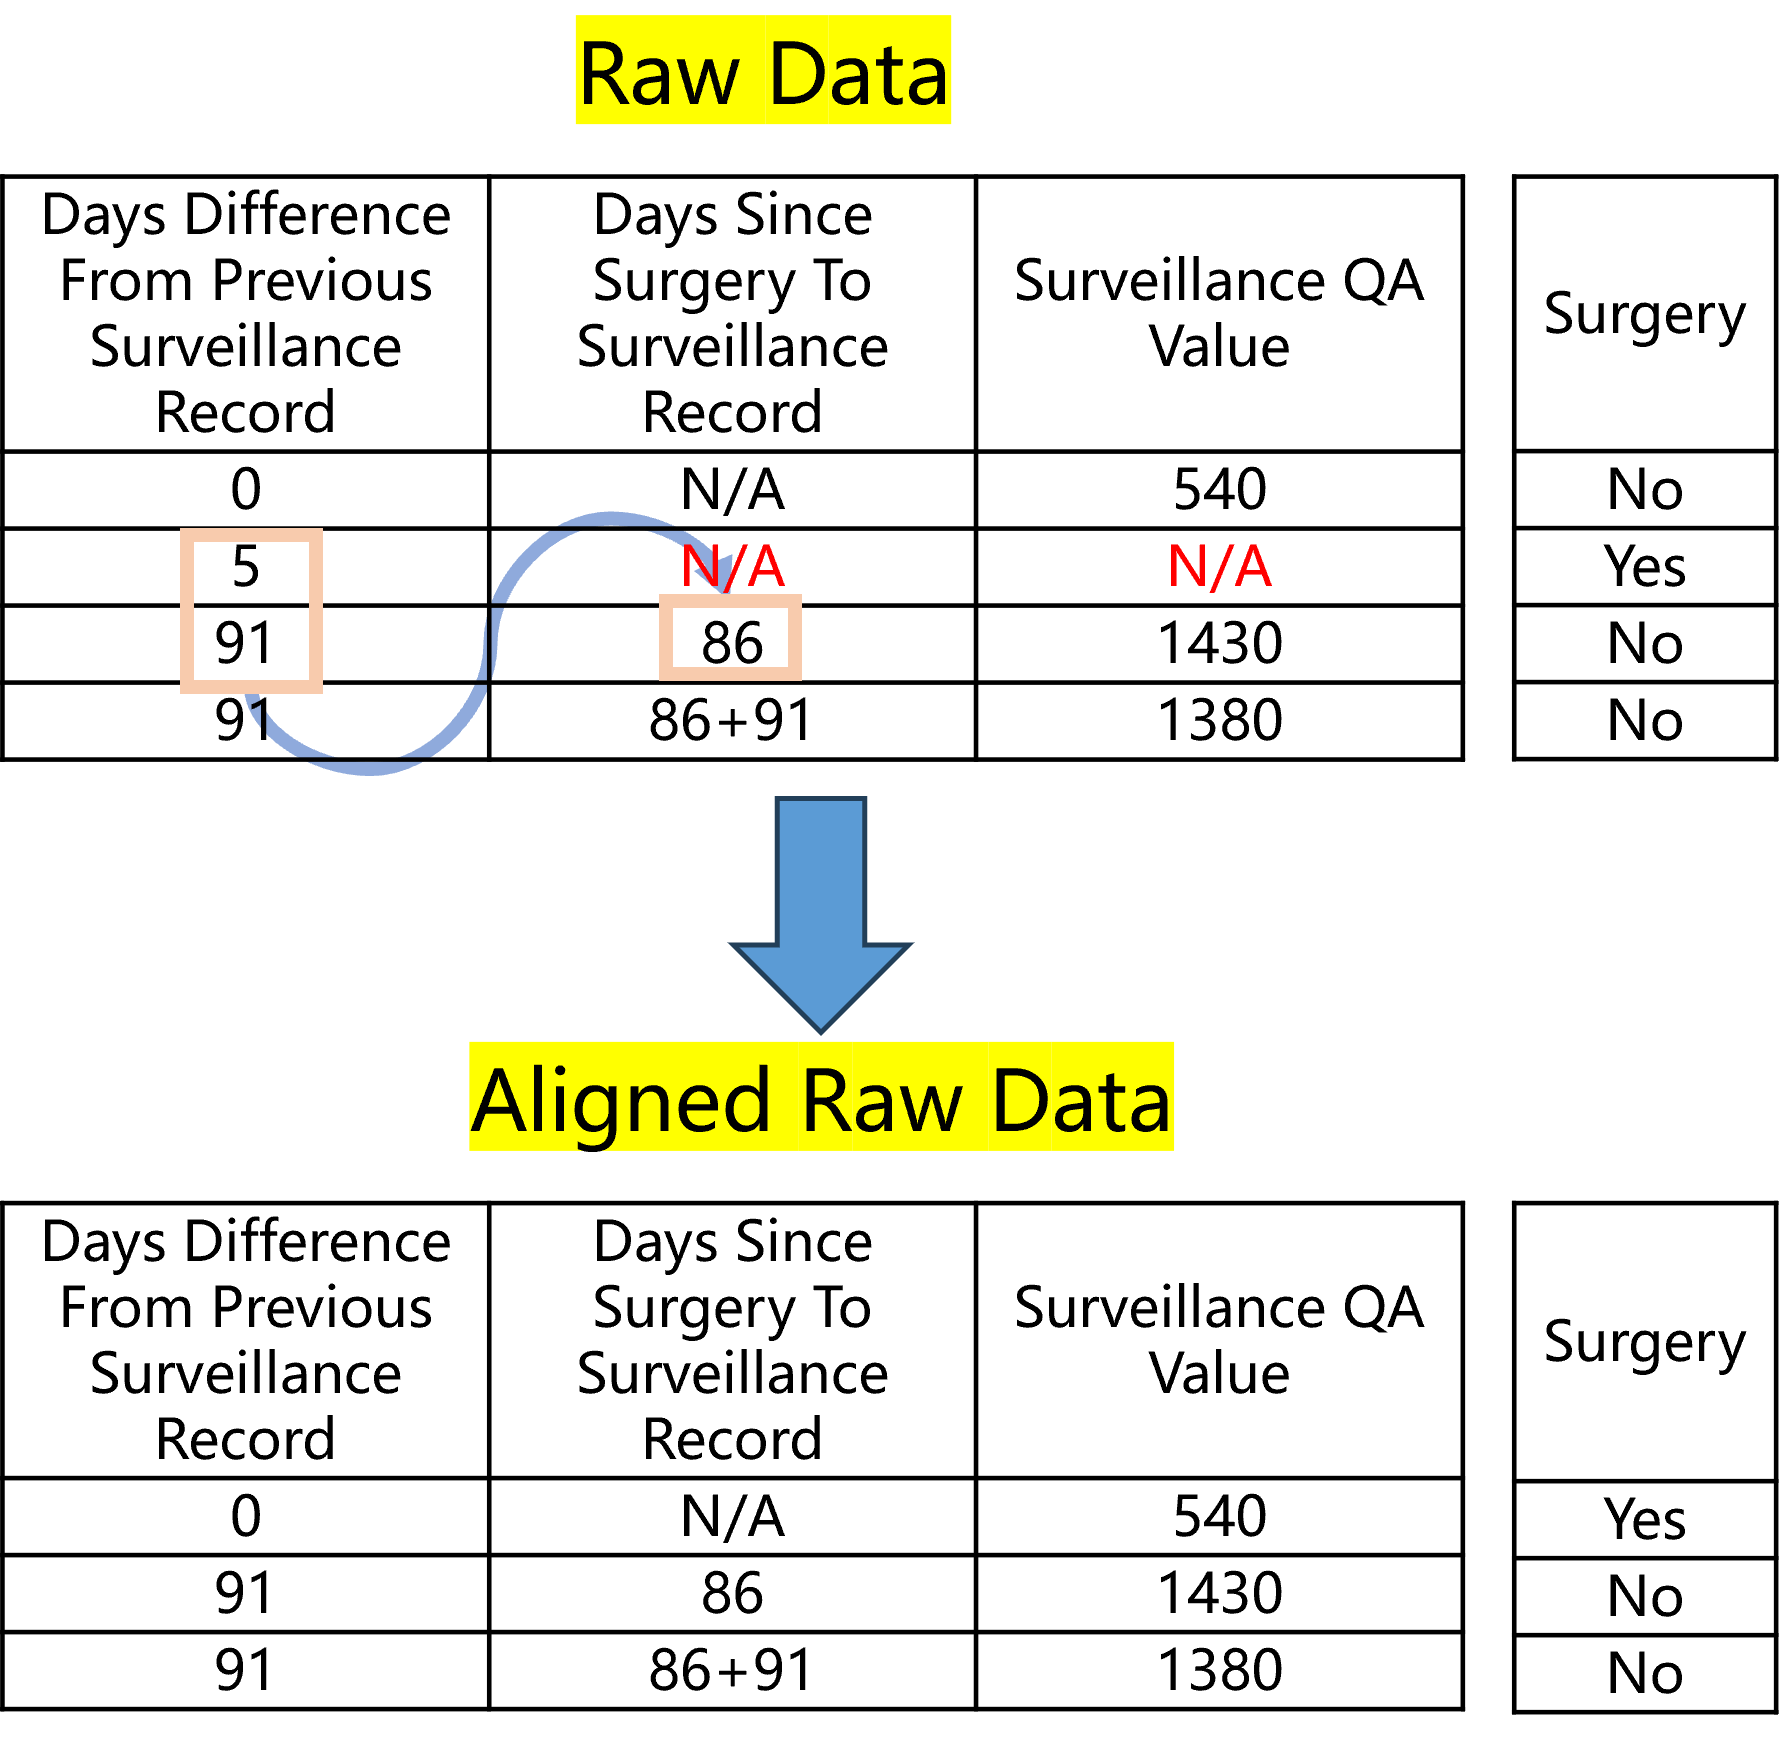
\includegraphics[width=\linewidth]{figures/Data Alignment.png}
        \caption{Data Alignment}
        \label{fig:pta-symptom}
    \end{subfigure}
    \caption{Data alignment process}
    \label{fig:combined}
\end{figure}

\subsection{Feature Creation}

As shown in Figure 4.3, the KDOQI (Kidney Disease Outcomes Quality Initiative) guidelines define three critical features related to vascular access dysfunction: (1) arteriovenous fistula (AVF) with a Qa value less than 400mL/min to 500 mL/min, (2) arteriovenous graft (AVG) with a Qa value less than 600 mL/min, and (3) cases where the Qa value is less than 1000 mL/min and has dropped by 25\%. These features serve as clinically significant indicators for evaluating the performance and functionality of vascular access. Inspired by these guidelines, additional features were created to enhance the model's ability to predict surgical outcomes. These newly created features capture variations in blood flow that may indicate vascular access dysfunction, aiming to provide the model with clinically meaningful variables that align with real-world diagnostic practices. 

\begin{figure}[H]
    \centering
    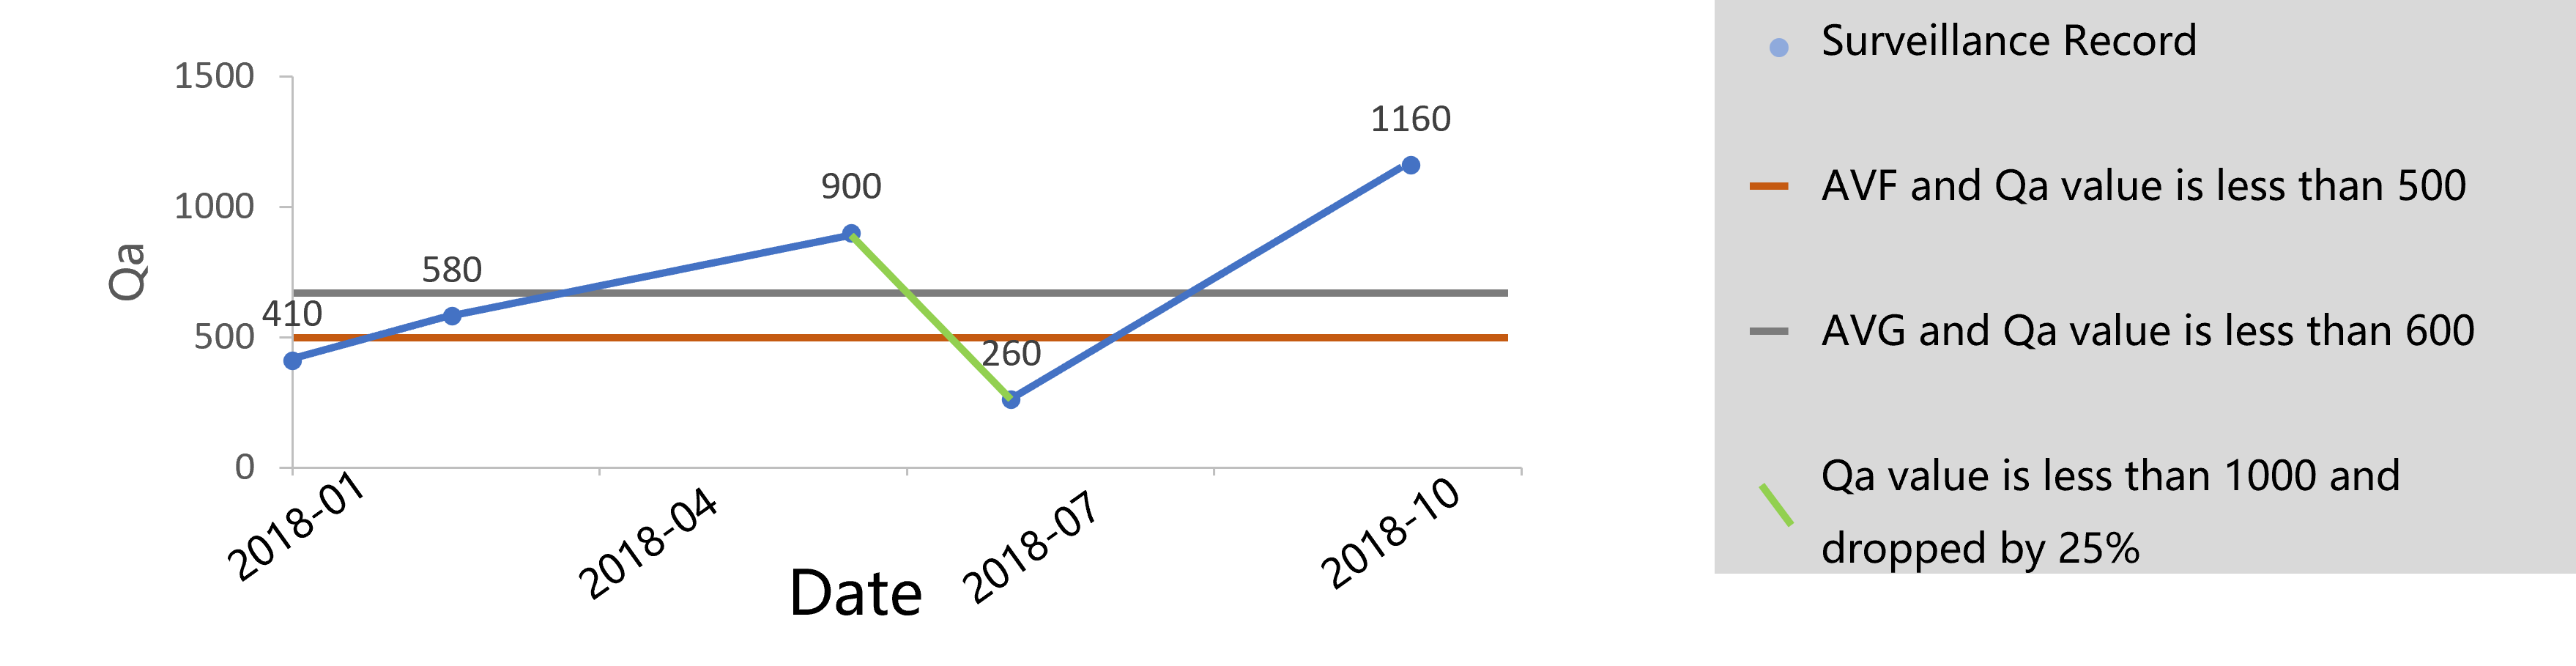
\includegraphics[width=1\linewidth]{figures/KDOQI guidelines.png}
    \caption{KDOQI guidelines feature method to determine whether to perform surgery}
    \label{fig:enter-label}
\end{figure}

To enhance the model's ability to capture historical trends and assess the current state of vascular access functionality, several new features were created. These features provide each sample with information from previous measurements, enabling the model to analyze temporal patterns and changes. The created features are as follows:

\begin{itemize}
    \item \textbf{Qa Value from the Previous Check}: This feature includes the Qa value recorded in the patient's most recent prior check, providing context on the patient's previous vascular access condition.
    \item \textbf{Previous Surgery Indicator}: A binary feature indicating whether a surgical procedure was performed during the previous check. This feature helps identify the impact of recent interventions on the current condition.
    \item \textbf{Slope of Qa Value Difference}: This feature calculates the slope of the Qa value difference between the current and previous measurements, normalized by the number of days elapsed since the last check. It represents the rate of change in Qa value over time, offering a quantitative measure of vascular access deterioration or improvement. The calculation process for this feature is illustrated in Figure 4.4.
    \item \textbf{Difference in Qa Values}: The absolute difference between the current and previous Qa values. This feature captures the magnitude of change in vascular access functionality between two consecutive checks.
\end{itemize}

\begin{figure}[H]
    \centering
    \includegraphics[width=1\linewidth]{figures/The slope of the A value difference between the current and previous measurements relative to the days elapsed since the previous check.png}
    \caption{The slope of the Qa value difference between the current and previous measurements relative to the days elapsed since the previous check}
    \label{fig:enter-label}
\end{figure}

By incorporating these newly created features, each sample is enriched with its historical context, enabling the model to assess trends and variations effectively. The slope and Qa value difference features, in particular, allow the model to detect significant changes in vascular access functionality, which are critical for predicting surgical needs.
\newpage
\section{Evaluation Metrics}

To comprehensively evaluate the performance of the proposed model, we designed an Extended Confusion Matrix that accounts for an additional category of predictions: Indeterminate. This extended framework enables a more nuanced evaluation of model performance, particularly in cases where predictions are inconclusive.

\subsection{Extended Confusion Matrix}

Figure 4.5 shows the Extended Confusion Matrix, which expands upon the traditional confusion matrix by including two new categories:

\begin{itemize}
    \item \textbf{IP (Indeterminate Positive)}: Actual positive cases predicted as indeterminate.
    \item \textbf{IN (Indeterminate Negative)}: Actual negative cases predicted as indeterminate.
\end{itemize}

\begin{figure}[H]
    \centering
    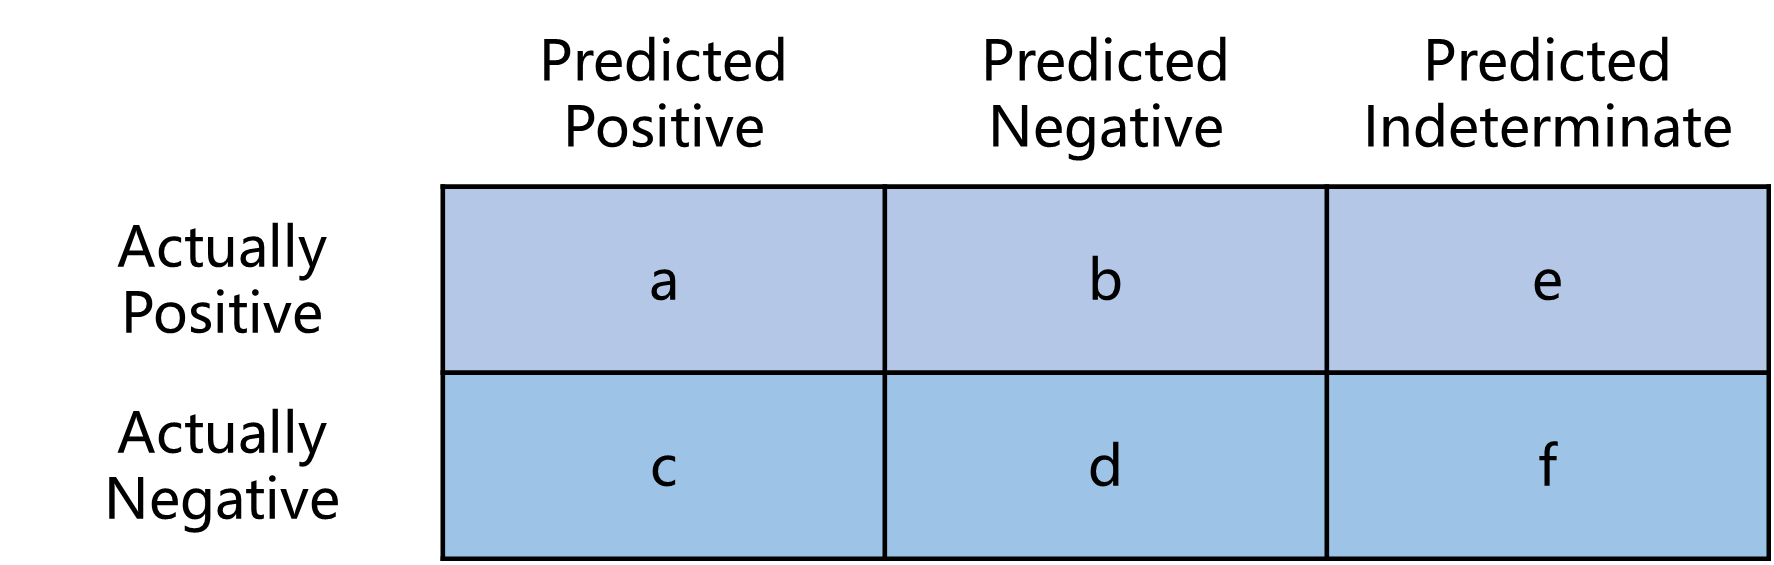
\includegraphics[width=0.6\linewidth]{figures/Extended confusion matrix.png}
    \caption{Extended confusion matrix. a: True Positive (TP), b: False Negative (FN), c: False Positive (FP), d: True Negative (TN), e: Indeterminate Positive (IP), f: Indeterminate Negative (IN)}
    \label{fig:enter-label}
\end{figure}

\subsection{Evaluation Metrics}

Based on Figure 4.5 the Extended Confusion Matrix, we derived several evaluation metrics to measure model performance, including both standard and indeterminacy-aware metrics:

\begin{itemize}
  \item \textbf{Standard Metrics}: 
    \begin{equation}
        Accuracy = \frac{a + d}{a + b + c + d}
    \end{equation}
    \begin{equation}
        PPV = \frac{a}{a + c}
    \end{equation}
    \begin{equation}
        NPV = \frac{d}{b + d}
    \end{equation}
  \item \textbf{Indeterminacy Metrics}: 
    \begin{equation}
        All = a + b + c + d + e + f
    \end{equation}
    \begin{equation}
        Error = \frac{b + c}{All}
    \end{equation}
    \begin{equation}
        Leakage = \frac{b}{All}
    \end{equation}
    \begin{equation}
        Overkill = \frac{c}{All}
    \end{equation}
    \begin{equation}
        Indeterminate = \frac{e + f}{All}
    \end{equation}
    \begin{equation}
        Imperfection = \frac{b + c + e + f}{All}
    \end{equation}
    \begin{equation}
        Indeterminate Recall = \frac{a + e}{a + b + e}
    \end{equation}
    \begin{equation}
        Harmonic\_Score = \frac{\frac{w_1'}{\exp\left(\frac{b}{All}\right)} + \frac{w_2'}{\exp\left(\frac{c}{All}\right)} + \frac{w_3'}{\exp\left(\frac{e + f}{All}\right)}}{3}
    \end{equation}
\end{itemize}

Positive Predictive Value (PPV) evaluates the proportion of predicted positive cases that are actually positive, emphasizing the model’s ability to minimize unnecessary interventions. Negative Predictive Value (NPV) measures the proportion of predicted negative cases that are truly negative, reducing the risk of missed diagnoses. Error Rate quantifies the proportion of all incorrect predictions, providing an overall misclassification rate. Beyond these standard metrics, Leakage Rate captures the proportion of actual positive cases classified as negative, highlighting the risk of failing to detect cases needing intervention, while Overkill Rate measures the proportion of actual negative cases classified as positive, addressing the tendency for over-treatment. Indeterminacy Rate reflects the proportion of predictions classified as indeterminate, enabling the model to flag ambiguous cases for further evaluation. Combining these, the Imperfection Rate aggregates the error and indeterminacy rates to assess the total proportion of samples either misclassified or marked as indeterminate. Additionally, Indeterminate Recall extends the traditional recall metric by including indeterminate positive cases, ensuring the model prioritizes identifying all potential positive cases. Finally, the Harmonic Score provides a balanced measure of leakage, overkill, and indeterminacy rates using weighted components, offering an integrated assessment of the model’s ability to minimize errors, reduce unnecessary interventions, and manage indeterminacy effectively. Together, these metrics form a comprehensive framework for evaluating both the predictive performance and reliability of the model.

\section{Experiment Setup}

In this study, we employed an ensemble learning approach by combining Decision Tree, Random Forest, and XGBoost models into a Soft Voting model. The Decision Tree serves as a base model, providing interpretability for feature impact; Random Forest enhances model robustness through the aggregation of predictions from multiple trees; and XGBoost further improves prediction accuracy with its efficient gradient boosting algorithm. The Soft Voting model integrates the predictions from these individual models using a weighted voting mechanism, achieving overall performance improvement and effectively handling the complexity and indeterminacy in the dataset.

All three models in the Soft Voting ensemble were used with default parameters, except for the \texttt{scale\_pos\_weight} parameter in XGBoost, which was set based on the ratio of patients requiring surgery to those not requiring surgery in the dataset. This adjustment was made to address the data imbalance and ensure the model accurately captured the underrepresented class. The experiments were conducted using a K-fold cross-validation approach with three iterations, and the final results were averaged for consistency. All computations and model training were performed on a high-performance NVIDIA Tesla V100 GPU to ensure efficiency.
\newpage

\section{Experiment Results}

This section summarizes the experimental results for the Arteriovenous Fistula (AVF) and Arteriovenous Graft (AVG) datasets under various parameter settings. By comparing the performance of the KDOQI guidelines with the proposed model, including scenarios where the model incorporates and excludes indeterminate classifications, we evaluate the advantages of our approach in improving diagnostic precision and managing indeterminacy. Key insights are derived from the results of the extended confusion matrix, ROC curves, and the evaluation metrics introduced earlier, highlighting the proposed model’s ability to provide robust and clinically meaningful predictions.

Figures 4.6 illustrate the relationship between the indeterminacy rate and the threshold parameter (\(\theta_{\mu}\)) for the AVF and AVG datasets, respectively. As the threshold increases, the proportion of samples classified as indeterminate decreases, reflecting the model's growing confidence in its predictions. For the AVF dataset, the indeterminacy rate drops from 50\% at a threshold of 0.75 to below 10\% at a threshold of 1.00, while the AVG dataset follows a similar trend, starting at 70\% and decreasing to under 10\%. The higher initial indeterminacy rate for the AVG dataset highlights the increased indeterminacy associated with its smaller sample size and higher proportion of surgical cases. These trends underscore the importance of threshold tuning to balance model confidence and sensitivity to indeterminate cases. A lower threshold captures more ambiguous samples, aiding cautious decision-making, while a higher threshold emphasizes definitive classifications, improving specificity. Based on these findings, we selected a threshold of 0.95, ensuring that the indeterminacy rate remains below 10\% for both datasets. This choice achieves a balance between minimizing indeterminate cases and maintaining high prediction confidence, aligning with the clinical need for precise yet cautious decision-making.

\begin{figure}[H]
    \centering
    \begin{subfigure}[b]{0.5\textwidth}
        \centering
        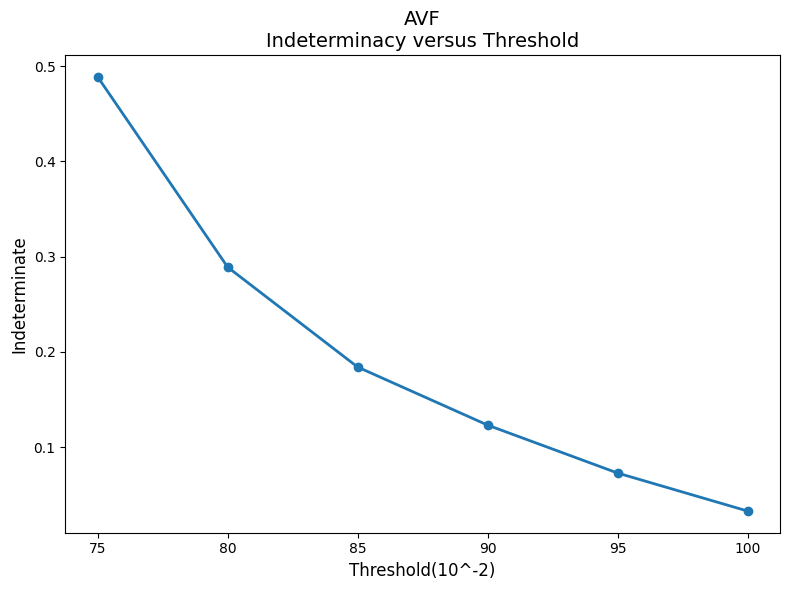
\includegraphics[width=\linewidth]{figures/AVF_Threshold changes used to determine output of indeterminacy.png}
        \caption{Indeterminacy Rate versus Threshold for the AVF Dataset}
        \label{fig:vascular-access}
    \end{subfigure}%
    \hfill
    \begin{subfigure}[b]{0.5\textwidth}
        \centering
        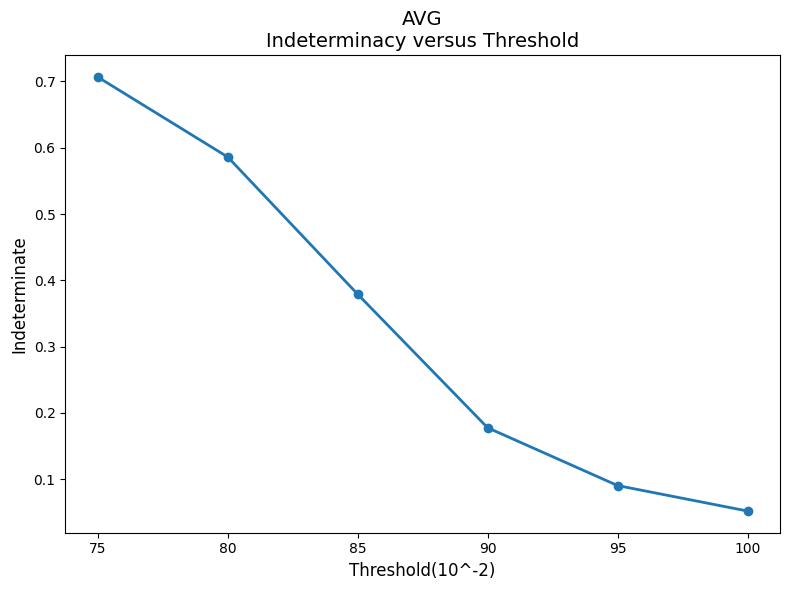
\includegraphics[width=\linewidth]{figures/AVG_Threshold changes used to determine output of indeterminacy.png}
        \caption{Indeterminacy Rate versus Threshold for the AVG Dataset}
        \label{fig:pta-symptom}
    \end{subfigure}
    \caption{Threshold changes used to determine output of indeterminacy}
    \label{fig:combined}
\end{figure}

\subsection{Arteriovenous Fistula Dataset}%AVF

The analysis of the Arteriovenous Fistula (AVF) dataset highlights the significant advantages of the proposed indeterminate-aware model in improving clinical decision-making and addressing indeterminacies in vascular access predictions. This section discusses the experimental results, parameter optimization, and model evaluation, emphasizing the practical implications of the findings.

The parameter settings for the model, determined using Bayesian optimization to maximize accuracy, are presented in Table 4.1. This optimization process identified the best combination of parameters to enhance the model’s predictive performance. 

\begin{table}[H]
    \centering
    \caption{The parameter settings in AVF Dataset}
    \renewcommand{\arraystretch}{1} % 調整行距
    \begin{tabular}[h]{lc} \hline 
        \multicolumn{2}{c}{Parameter Settings} \\ \hline
        Number of estimation times: \(n\) & 10\\ 
        Threshold used to determine output of indeterminacy: \(\theta_{\mu}\) &  0.95\\ 
        Noise mean: \(\mu\) & 0\\ 
        Noise variance: \(\sigma^2\) & 100\\
        Weight of estimator: \(W=[w_{1},w_{2},w_{3}]\) & [1,1,1]\\
        Weight of harmonic score: \(W'=[w_1',w_2',w_3']\) & [1,1,1] \\ \hline 
    \end{tabular}
    \label{tab:Experimental_Config_AVF}
\end{table}

Figure 4.7 illustrates the distribution of the AVF dataset. Out of 4,991 cases, 546 (10.9\%) required PTA interventions, while 4,445 (89.1\%) did not undergo surgery. This imbalance highlights the dataset’s focus on monitoring cases to avoid unnecessary surgical procedures.

\begin{figure}[H]
    \centering
    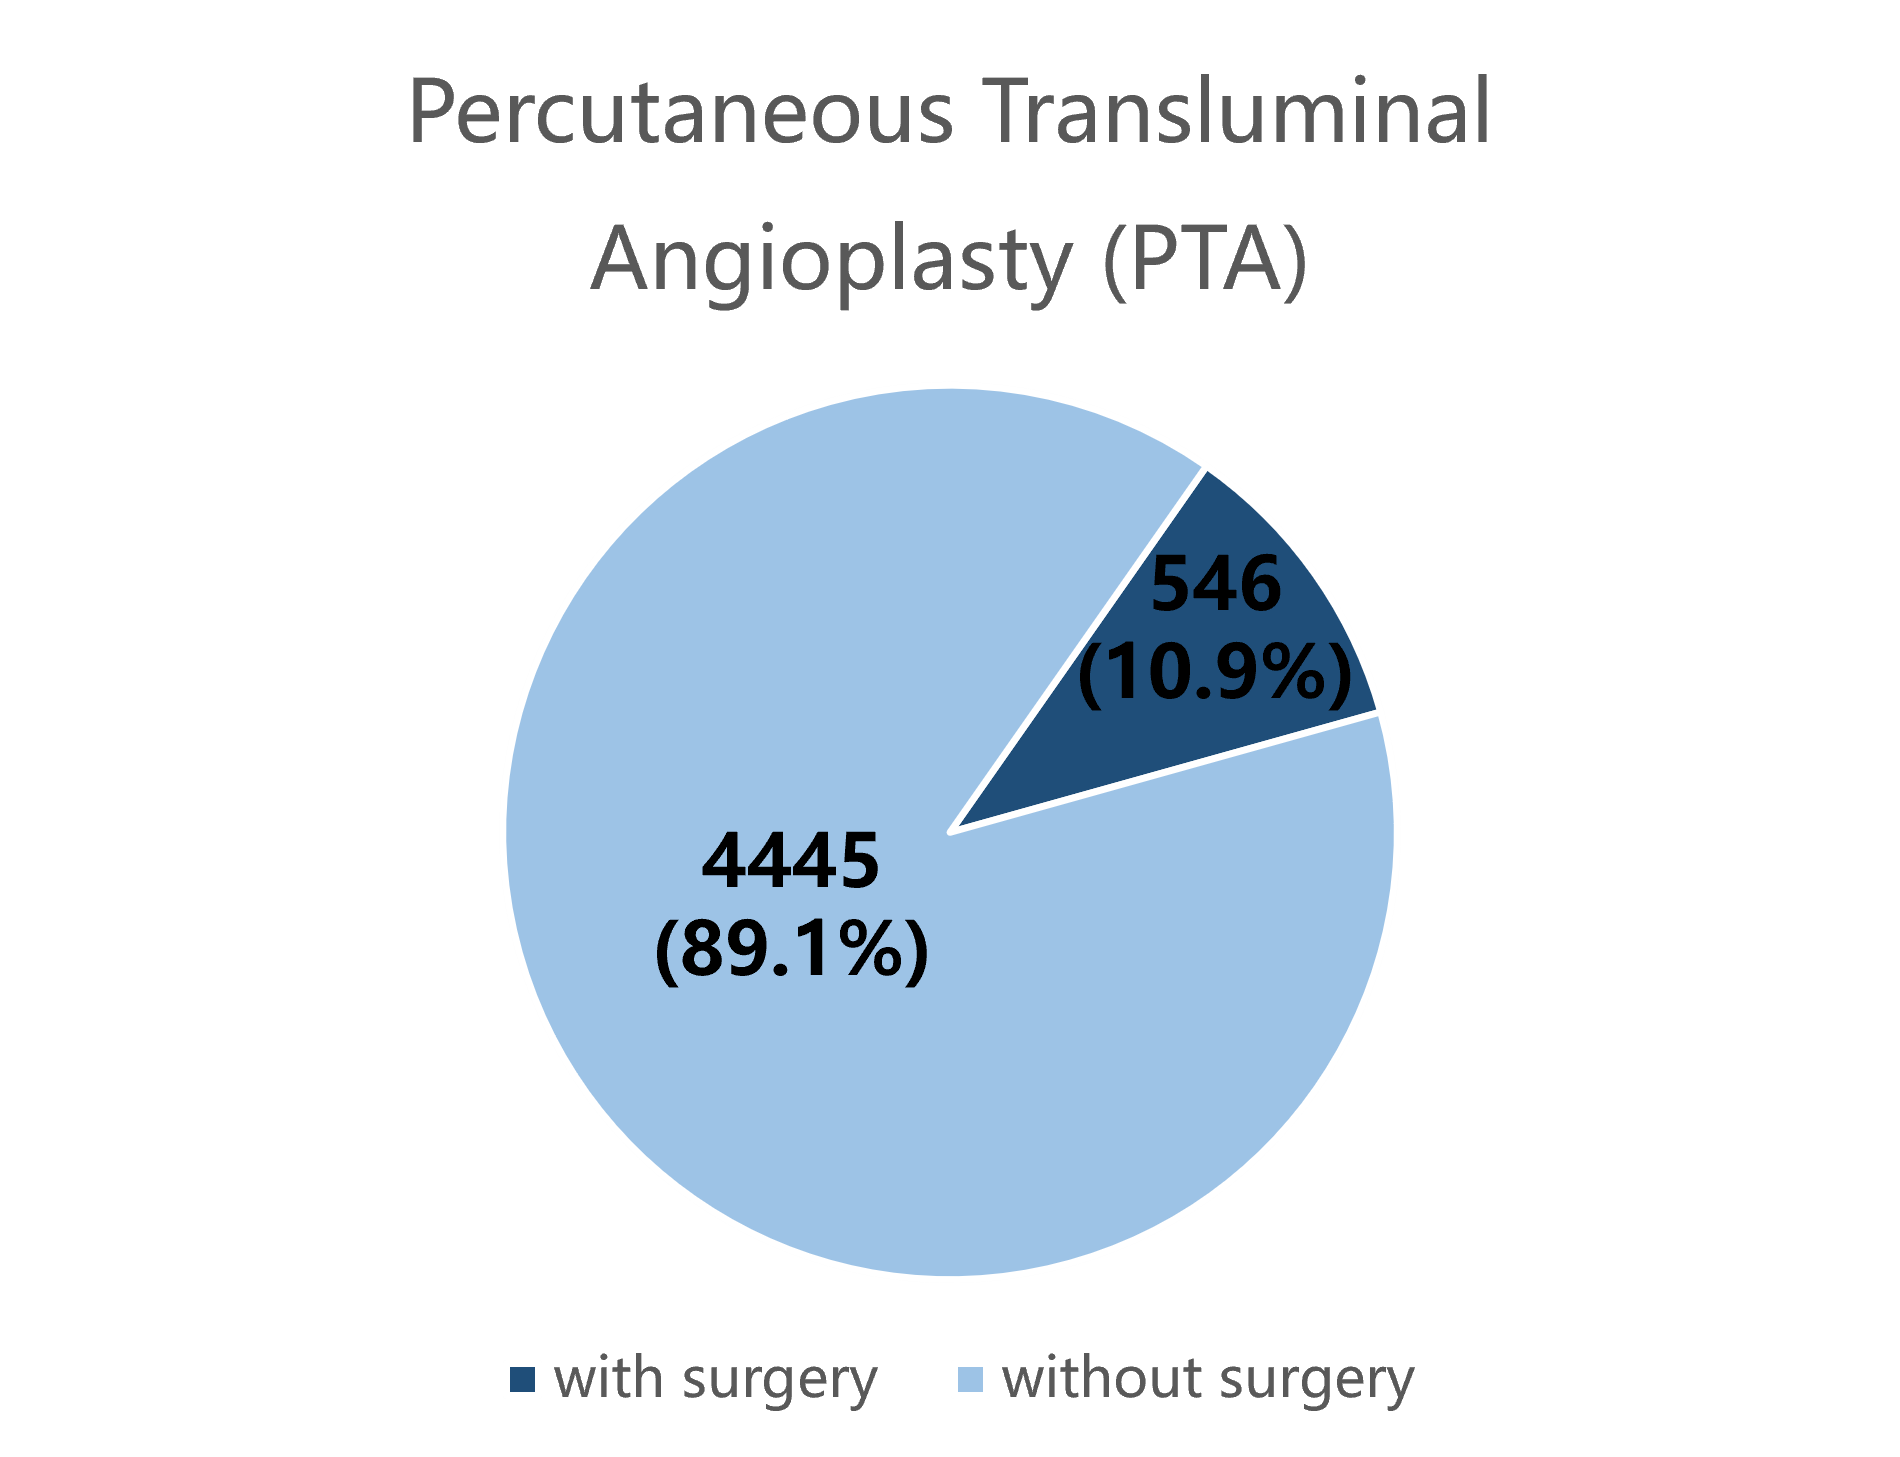
\includegraphics[width=0.7\linewidth]{figures/AVF data distribution.png}
    \caption{AVF data distribution}
    \label{fig:enter-label}
\end{figure}

The comparison of evaluation metrics is detailed in Table 4.2, 4.3, and 4.4, showing results for the KDOQI guidelines, our proposed model without indeterminate classification, and our model with indeterminate classification:

\begin{table}[h]
\centering
% [] 顯示在 list of tables 的文字
% {} 顯示在表格上方的文字
\caption[AVF Dataset Standard Metrics of Baseline, Our Method(Without indeterminate), Our Method(indeterminate)]{AVF Dataset Standard Metrics of Baseline, Our Method(Without indeterminate), Our Method(indeterminate)}
\label{Standard Metrics AVF}
\begin{tabular}{ccccc}
\toprule[1.1pt]
                      & Accuracy & PPV & NPV \\
\midrule[1.1pt]
\multirow{1}{*}{Baseline} & 0.872 ± 0.001 &0.394 ± 0.011 & 0.918 ± 0.003 & \\
\midrule
\multirow{1}{*}{Our Method(Without indeterminate)} & 0.895 ± 0.004 & 0.589 ± 0.028 & 0.904 ± 0.002 \\
\midrule
\multirow{1}{*}{Our Method(indeterminate)} & \textbf{0.913 ± 0.001} & \textbf{0.841 ± 0.043} & 0.914 ± 0.001 \\

\bottomrule[1.1pt]
\end{tabular}
\end{table}


\begin{table}[h]
\centering
% [] 顯示在 list of tables 的文字
% {} 顯示在表格上方的文字
\caption[AVF Dataset Indeterminacy Metrics (I) of Baseline, Our Method(Without indeterminate), Our Method(indeterminate)]{AVF Dataset Indeterminacy Metrics (I) of Baseline, Our Method(Without indeterminate), Our Method(indeterminate)}
\label{Indeterminacy Metrics(I) AVF}
\begin{tabular}{ccccc}
\toprule[1.1pt]
                      & Error & Leakage & Overkill & Indeterminate \\
\midrule[1.1pt]
\multirow{1}{*}{Baseline} & 0.129 ± 0.01 & 0.078 ± 0.012 & 0.051 ± 0.031 & - \\
\midrule
\multirow{1}{*}{Our Method(Without indeterminate)} & 0.105 ± 0.004 & 0.093 ± 0.001 & 0.011 ± 0.003 & - \\
\midrule
\multirow{1}{*}{Our Method(indeterminate)} & \textbf{0.081 ± 0.002} & \textbf{0.08 ± 0.002} & \textbf{0.002 ± 0.002} & 0.073 ± 0.027 \\

\bottomrule[1.1pt]
\end{tabular}
\end{table}

\begin{table}[H]
\centering
% [] 顯示在 list of tables 的文字
% {} 顯示在表格上方的文字
\caption[AVF Dataset Indeterminacy Metrics (II) of Baseline, Our Method(Without indeterminate), Our Method(indeterminate)]{AVF Dataset Indeterminacy Metrics (II) of Baseline, Our Method(Without indeterminate), Our Method(indeterminate)}
\label{Indeterminacy Metrics(II) AVF}
\begin{tabular}{ccccc}
\toprule[1.1pt]
                      & Imperfection & Indeterminate recall & Harmonic score \\
\midrule[1.1pt]
\multirow{1}{*}{Baseline} & 0.129 ± 0.01 & 0.261 ± 0.039 & 0.958 ± 0.002\\
\midrule
\multirow{1}{*}{Our Method(Without indeterminate)} & 0.105 ± 0.004 & 0.146 ± 0.014 & 0.967 ± 0.001 \\
\midrule
\multirow{1}{*}{Our Method(indeterminate)} & 0.154 ± 0.021 & \textbf{0.292 ± 0.03} & 0.951 ± 0.008 \\

\bottomrule[1.1pt]
\end{tabular}
\end{table}

The extended confusion matrix, as shown in Figure 4.8, provides deeper insights into how the model handles ambiguous cases. Unlike the KDOQI guidelines, which classify all cases as either positive or negative, the indeterminate-aware model assigns indeterminate cases to a separate "Indeterminate" category. This approach prevents overly confident misclassifications, particularly for borderline cases where the probability distributions lack clear separation. By reallocating indeterminate predictions, the model reduces the likelihood of errors, ensuring a more cautious and clinically meaningful decision-making process.

\begin{figure}[H]
    \centering
    \begin{subfigure}[b]{0.5\textwidth}
        \centering
        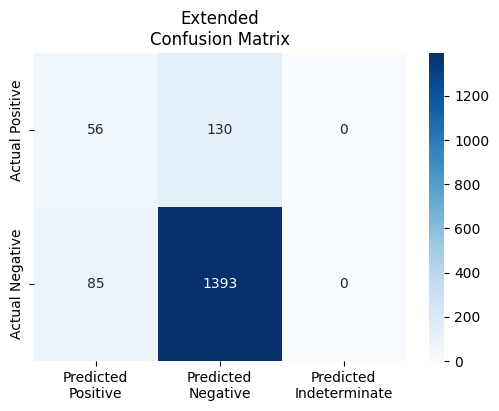
\includegraphics[width=\linewidth]{figures/kdoqi_AVF.png}
        \caption{baseline}
        \label{fig:vascular-access}
    \end{subfigure}
    
    \vspace{1em} % 增加垂直空間

    \begin{subfigure}[b]{0.5\textwidth}
        \centering
        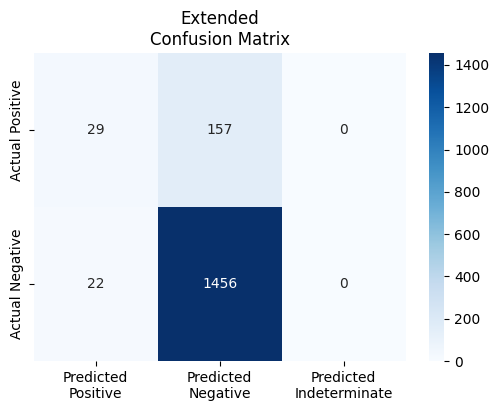
\includegraphics[width=\linewidth]{figures/without_AVF.png}
        \caption{Our Method (Without indeterminate)}
        \label{fig:pta-symptom-method1}
    \end{subfigure}%
    \hfill
    \begin{subfigure}[b]{0.5\textwidth}
        \centering
        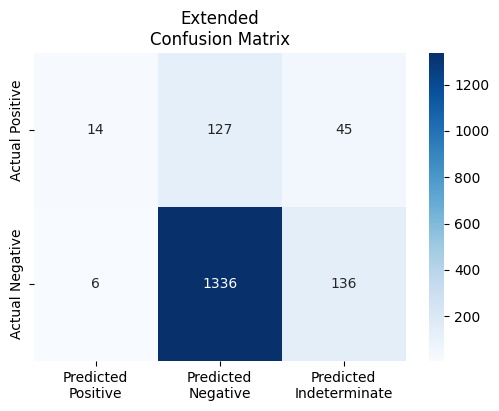
\includegraphics[width=\linewidth]{figures/with_AVF.png}
        \caption{Our Method (Indeterminate)}
        \label{fig:pta-symptom-method2}
    \end{subfigure}

    \caption{AVF Dataset Extended Confusion Matrix}
    \label{fig:combined}
\end{figure}


The ROC curve comparisons, as presented in Figure 4.9, further validate the proposed model's superior discriminative ability. The baseline KDOQI guidelines achieved an AUC of 0.62, reflecting its limited predictive capability. In contrast, the proposed model without indeterminate classification improved to an AUC of 0.73, and the inclusion of indeterminate classifications further enhanced the AUC to 0.76. This progression demonstrates that the model's ability to distinguish between positive and negative cases improves significantly when indeterminacy is explicitly accounted for.

\begin{figure}[H]
    \centering
    \begin{subfigure}[b]{0.5\textwidth}
        \centering
        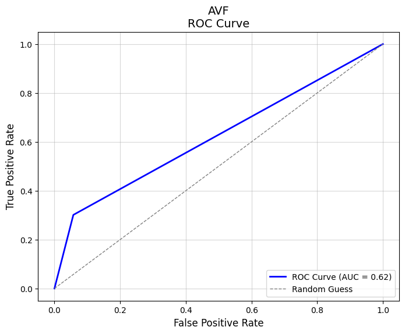
\includegraphics[width=\linewidth]{figures/AVF_baseline_roc.png}
        \caption{baseline}
        \label{fig:vascular-access-roc}
    \end{subfigure}
    
    \vspace{1em} % 增加垂直空間

    \begin{subfigure}[b]{0.5\textwidth}
        \centering
        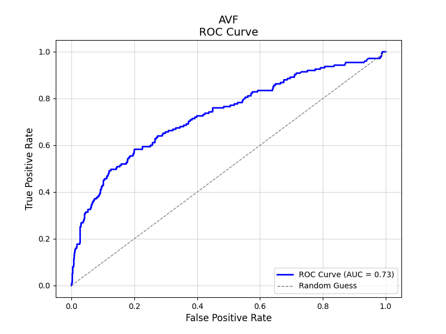
\includegraphics[width=\linewidth]{figures/AVF_method1_roc.png}
        \caption{Our Method (Without indeterminate)}
        \label{fig:pta-symptom-method1-roc}
    \end{subfigure}%
    \hfill
    \begin{subfigure}[b]{0.5\textwidth}
        \centering
        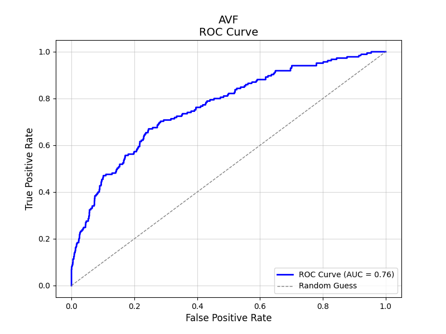
\includegraphics[width=\linewidth]{figures/AVF_method2_roc.png}
        \caption{Our Method (Indeterminate)}
        \label{fig:pta-symptom-method2-roc}
    \end{subfigure}

    \caption{AVF Dataset ROC Curve}
    \label{fig:combined}
\end{figure}

The results from the AVF dataset illustrate the effectiveness of incorporating indeterminate classifications into the prediction framework. The proposed model not only surpasses the KDOQI guidelines in terms of accuracy and precision but also introduces a critical layer of indeterminacy management, which is essential for clinical applications. By balancing standard predictive metrics with indeterminacy-specific measures, the model ensures that ambiguous cases are flagged for further review, reducing the risk of misdiagnoses and unnecessary interventions. These findings underscore the clinical potential of the indeterminate-aware approach for managing vascular access in hemodialysis patients.

\subsection{Arteriovenous Graft Dataset}%AVG

The analysis of the Arteriovenous Graft (AVG) dataset provides complementary insights into the proposed model's performance, particularly in a dataset with fewer samples and a higher proportion of surgical interventions compared to the AVF dataset. This section discusses the dataset characteristics, model evaluation, and the implications of the results.

As shown in Table 4.5, the parameters for the AVG dataset were optimized using Bayesian optimization, which maximized accuracy. 

\begin{table}[H]
    \centering
    \caption{The parameter settings in AVG Dataset}
    \renewcommand{\arraystretch}{1} % 調整行距
    \begin{tabular}[h]{lc} \hline 
        \multicolumn{2}{c}{Parameter Settings} \\ \hline
        Number of estimation times: \(n\) & 10\\ 
        Threshold used to determine output of indeterminacy: \(\theta_{\mu}\) &  0.95\\ 
        Noise mean: \(\mu\) & 0\\ 
        Noise variance: \(\sigma^2\) & 80\\
        Weight of estimator: \(W=[w_{1},w_{2},w_{3}]\) & [1,1,1]\\
        Weight of harmonic score: \(W'=[w_1',w_2',w_3']\) & [1,1,1] \\ \hline 
    \end{tabular}
    \label{tab:Experimental_Config_AVG}
\end{table}

The AVG dataset comprises a total of 869 records, significantly fewer than the 4,991 records in the AVF dataset, as shown in Figure 4.10. Among these records, 218 (25.1\%) involve PTA interventions, while 651 (74.9\%) represent non-surgical cases. The higher proportion of surgical cases in AVG compared to AVF (10.9\%) aligns with clinical observations that AVG is often associated with shorter durability and higher complication rates, necessitating more frequent interventions.

\begin{figure}[H]
    \centering
    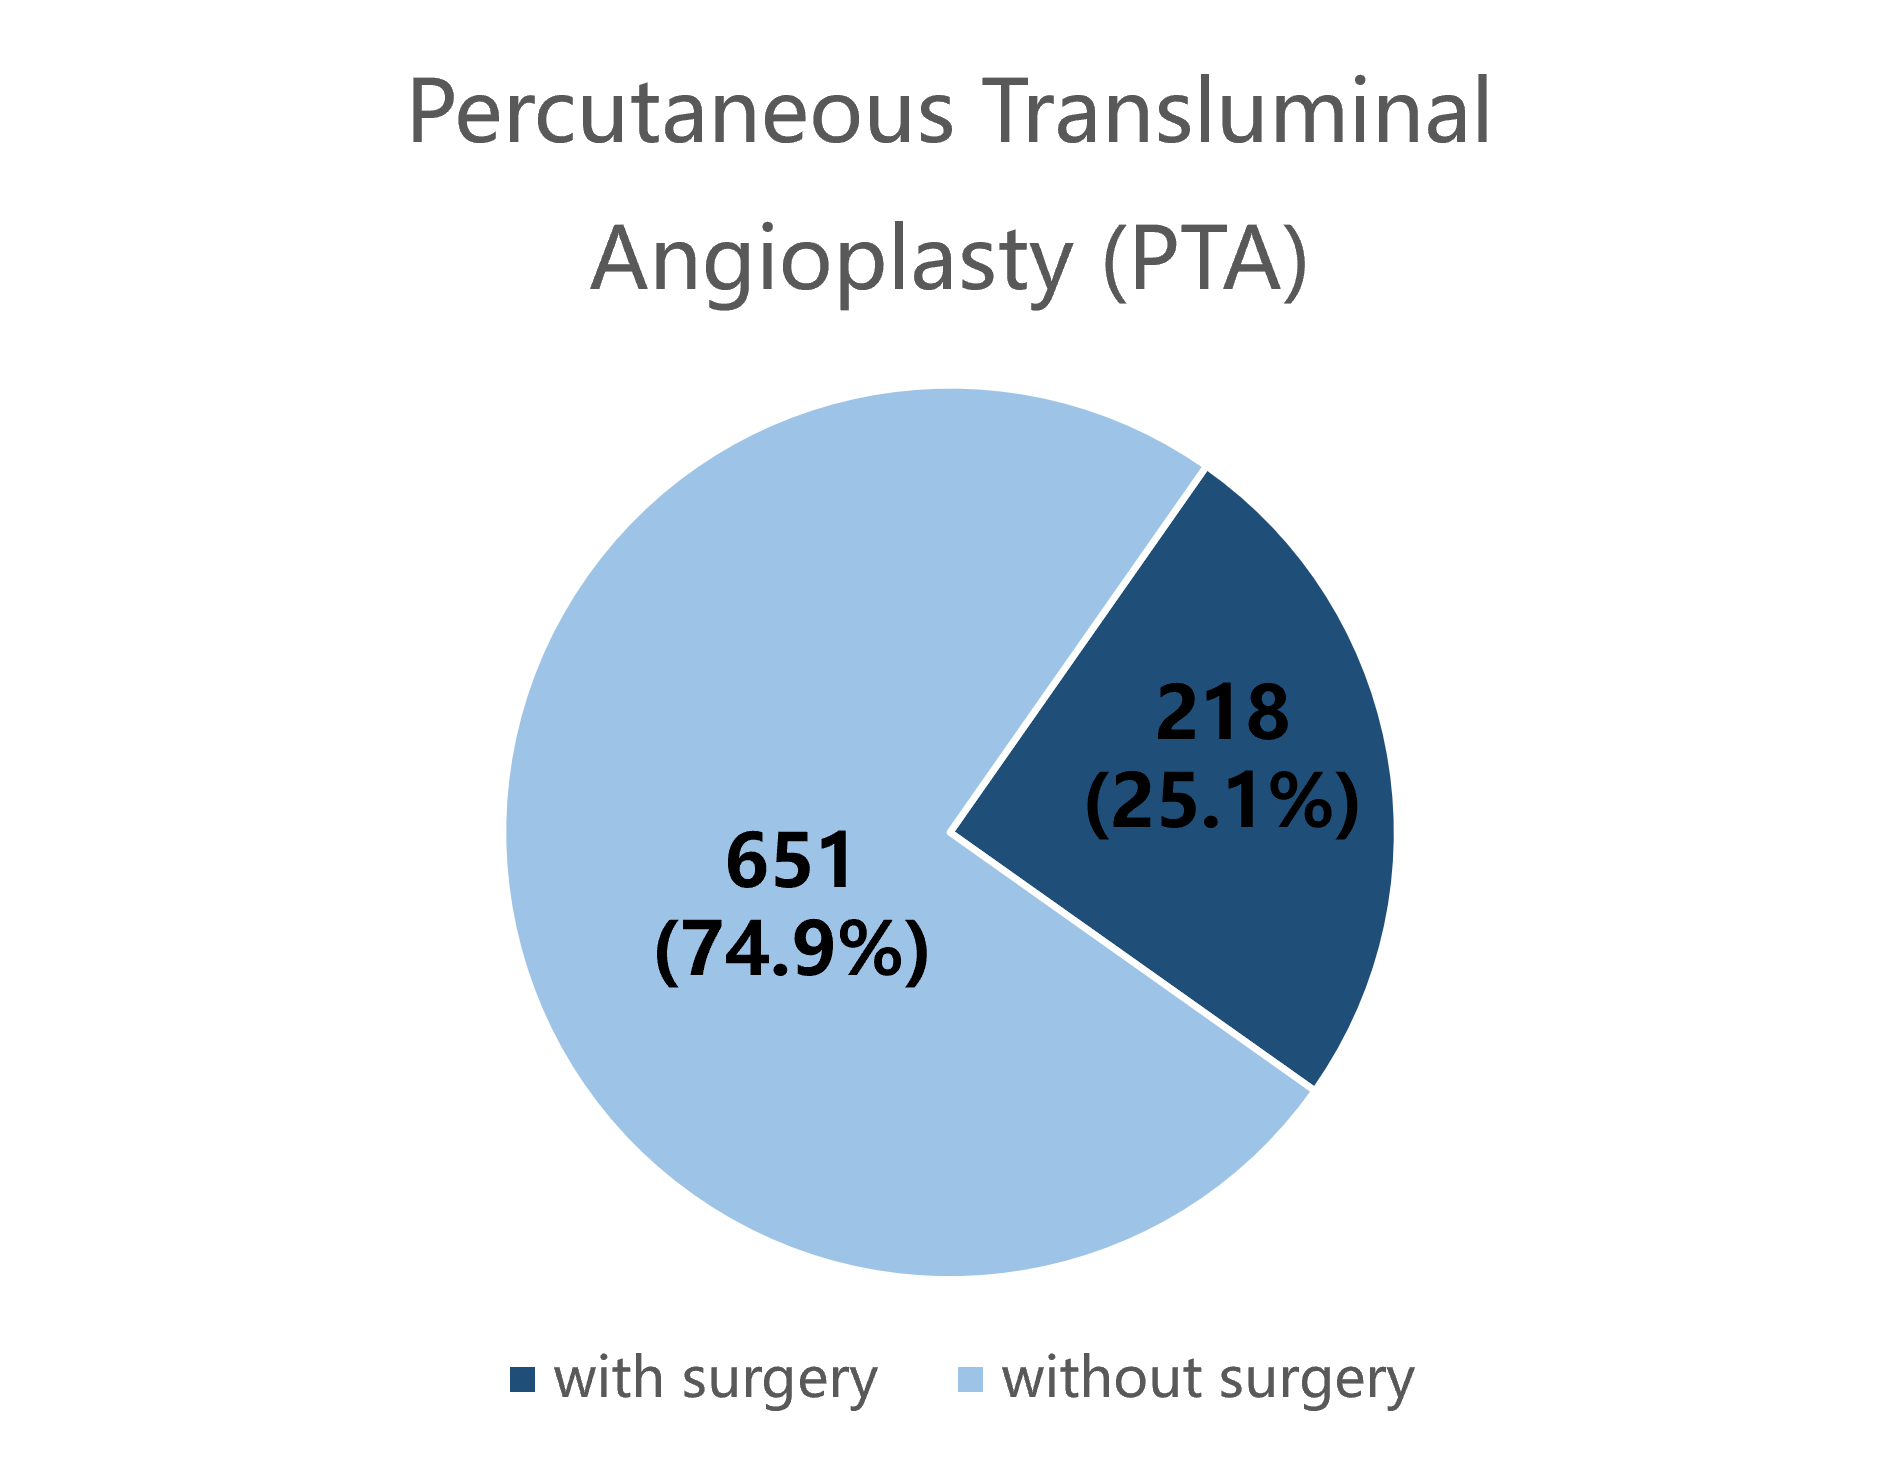
\includegraphics[width=0.7\linewidth]{figures/AVG data distribution.png}
    \caption{AVG data distribution}
    \label{fig:enter-label}
\end{figure}

Tables 4.6, 4.7, and 4.8 show the results of the comparison of metrics between KDOQI guidelines and our method on the AVG dataset.

\begin{table}[h]
\centering
% [] 顯示在 list of tables 的文字
% {} 顯示在表格上方的文字
\caption[AVG Dataset Standard Metrics of Baseline, Our Method(Without indeterminate), Our Method(indeterminate)]{AVG Dataset Standard Metrics of Baseline, Our Method(Without indeterminate), Our Method(indeterminate)}
\label{Standard Metrics AVG}
\begin{tabular}{ccccc}
\toprule[1.1pt]
                      & Accuracy & PPV & NPV \\
\midrule[1.1pt]
\multirow{1}{*}{Baseline} & 0.791 ± 0.018 &0.685 ± 0.044 & 0.809 ± 0.026 & \\
\midrule
\multirow{1}{*}{Our Method(Without indeterminate)} & 0.765 ± 0.023 & 0.695 ± 0.045 & 0.788 ± 0.028 \\
\midrule
\multirow{1}{*}{Our Method(indeterminate)} & \textbf{0.818 ± 0.019} & \textbf{0.74 ± 0.137} & \textbf{0.828 ± 0.031} \\

\bottomrule[1.1pt]
\end{tabular}
\end{table}


\begin{table}[h]
\centering
% [] 顯示在 list of tables 的文字
% {} 顯示在表格上方的文字
\caption[AVG Dataset Indeterminacy Metrics (I) of Baseline, Our Method(Without indeterminate), Our Method(indeterminate)]{AVG Dataset Indeterminacy Metrics (I) of Baseline, Our Method(Without indeterminate), Our Method(indeterminate)}
\label{Indeterminacy Metrics(I) AVG}
\begin{tabular}{ccccc}
\toprule[1.1pt]
                      & Error & Leakage & Overkill & Indeterminate \\
\midrule[1.1pt]
\multirow{1}{*}{Baseline} & 0.208 ± 0.032 & 0.186 ± 0.011 & 0.048 ± 0.016 & - \\
\midrule
\multirow{1}{*}{Our Method(Without indeterminate)} & 0.235 ± 0.023 & 0.19 ± 0.027 & 0.032 ± 0.017 & - \\
\midrule
\multirow{1}{*}{Our Method(indeterminate)} & \textbf{0.147 ± 0.017} & \textbf{0.128 ± 0.025} & \textbf{0.02 ± 0.011} & 0.192 ± 0.007 \\

\bottomrule[1.1pt]
\end{tabular}
\end{table}

\begin{table}[H]
\centering
% [] 顯示在 list of tables 的文字
% {} 顯示在表格上方的文字
\caption[AVG Dataset Indeterminacy Metrics (II) of Baseline, Our Method(Without indeterminate), Our Method(indeterminate)]{AVG Dataset Indeterminacy Metrics (II) of Baseline, Our Method(Without indeterminate), Our Method(indeterminate)}
\label{Indeterminacy Metrics(II) AVG}
\begin{tabular}{ccccc}
\toprule[1.1pt]
                      & Imperfection & Indeterminate recall & Harmonic score \\
\midrule[1.1pt]
\multirow{1}{*}{Baseline} & 0.208 ± 0.032 & 0.262 ± 0.07 & 0.908 ± 0.018\\
\midrule
\multirow{1}{*}{Our Method(Without indeterminate)} & 0.235 ± 0.023 & 0.247 ± 0.059 & 0.928 ± 0.013 \\
\midrule
\multirow{1}{*}{Our Method(indeterminate)} & 0.34 ± 0.011 & \textbf{0.496 ± 0.059} & 0.895 ± 0.013 \\

\bottomrule[1.1pt]
\end{tabular}
\end{table}

The extended confusion matrix in Figure 4.11 shows how the proposed model reallocates a significant proportion of indeterminate predictions to the "Indeterminate" category. Compared to AVF, the higher surgical proportion in AVG is evident in the relative distribution of predicted positive and negative cases. The indeterminate-aware approach ensures that borderline cases are cautiously flagged, avoiding overconfidence in predictions.

\begin{figure}[H]
    \centering
    \begin{subfigure}[b]{0.5\textwidth}
        \centering
        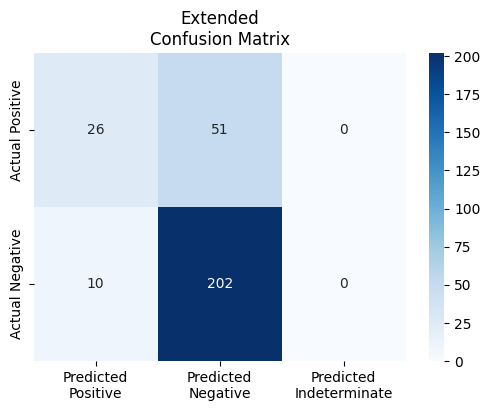
\includegraphics[width=\linewidth]{figures/kdoqi_AVG.png}
        \caption{baseline}
        \label{fig:vascular-access}
    \end{subfigure}
    
    \vspace{1em} % 增加垂直空間

    \begin{subfigure}[b]{0.5\textwidth}
        \centering
        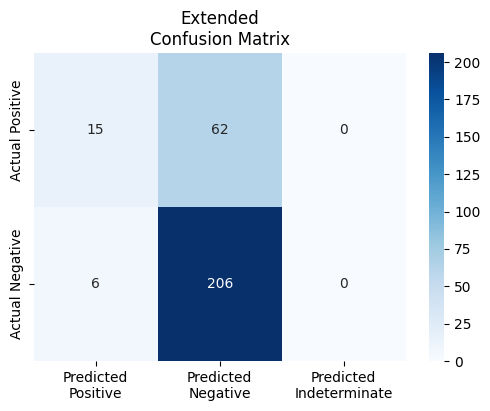
\includegraphics[width=\linewidth]{figures/without_AVG.png}
        \caption{Our Method (Without indeterminate)}
        \label{fig:pta-symptom-method1}
    \end{subfigure}%
    \hfill
    \begin{subfigure}[b]{0.5\textwidth}
        \centering
        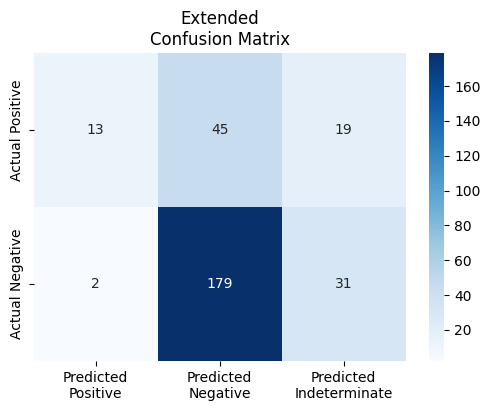
\includegraphics[width=\linewidth]{figures/with_AVG.png}
        \caption{Our Method (Indeterminate)}
        \label{fig:pta-symptom-method2}
    \end{subfigure}

    \caption{AVG Dataset Extended Confusion Matrix}
    \label{fig:combined}
\end{figure}

The ROC curve analysis, illustrated in Figure 4.12, shows the progression of AUC values across configurations. The baseline KDOQI guidelines achieved an AUC of 0.62, reflecting its limited predictive capability. The proposed model without indeterminate classification achieved an AUC of 0.64, while the inclusion of indeterminate classifications further improved the AUC to 0.73. These results demonstrate that explicitly accounting for indeterminacy enhances the model’s ability to distinguish between positive and negative cases.

\begin{figure}[H]
    \centering
    \begin{subfigure}[b]{0.5\textwidth}
        \centering
        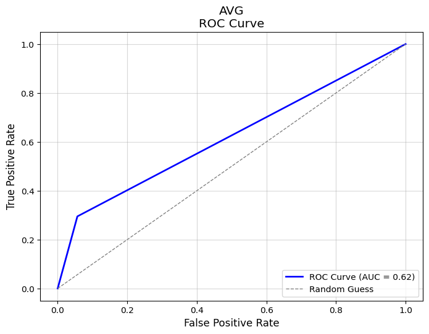
\includegraphics[width=\linewidth]{figures/AVG_baseline_roc.png}
        \caption{baseline}
        \label{fig:vascular-access-roc}
    \end{subfigure}
    
    \vspace{1em} % 增加垂直空間

    \begin{subfigure}[b]{0.5\textwidth}
        \centering
        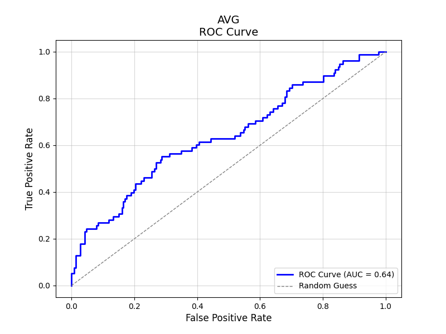
\includegraphics[width=\linewidth]{figures/AVG_method1_roc.png}
        \caption{Our Method (Without indeterminate)}
        \label{fig:pta-symptom-method1-roc}
    \end{subfigure}%
    \hfill
    \begin{subfigure}[b]{0.5\textwidth}
        \centering
        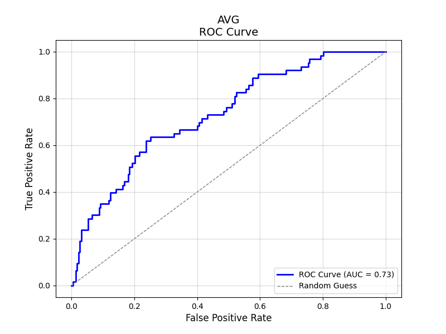
\includegraphics[width=\linewidth]{figures/AVG_method2_roc.png}
        \caption{Our Method (Indeterminate)}
        \label{fig:pta-symptom-method2-roc}
    \end{subfigure}

    \caption{AVG Dataset ROC Curve}
    \label{fig:combined}
\end{figure}

In comparison to the AVF dataset, the AVG dataset presents unique challenges due to its smaller size and higher surgical intervention rate. Despite these differences, the proposed indeterminate-aware model consistently outperformed both the KDOQI guidelines and the model without indeterminate classifications. The results emphasize the model’s adaptability and robustness, making it a valuable tool for supporting clinical decision-making in vascular access management.